\documentclass[11pt,a4paper]{article}
\usepackage[T1]{fontenc}
\usepackage[utf8]{inputenc}
\usepackage{lmodern,microtype}
\usepackage{amsmath,amssymb,amsthm,mathtools,bm}
\usepackage{booktabs,array,tabularx,longtable}
\usepackage{graphicx,float,caption}
\usepackage{xcolor}
\usepackage[margin=20mm]{geometry}
\usepackage{enumitem,fancyhdr}
\usepackage[hidelinks,unicode=true]{hyperref}
\hypersetup{
 pdftitle={FIN ST178--ST189: Layered Compression Visibility and Validated Continuation},
 pdfauthor={Krzysztof Żuchowski},
 pdfsubject={Analytical, interval, and computational execution of FIN programs ST178--ST189},
 pdfkeywords={FIN, fractal information, layered compression, sufficient statistic, visibility spectrum, data processing, state-dependent interaction, fold continuation, detailed balance, hidden Markov model, quantum bath}
}
\setlength{\parindent}{0pt}
\setlength{\parskip}{0.48em}
\setlength{\emergencystretch}{2em}
\setlength{\headheight}{14pt}
\setlist[itemize]{leftmargin=1.55em,itemsep=0.14em,topsep=0.2em}
\setlist[enumerate]{leftmargin=1.75em,itemsep=0.14em,topsep=0.2em}
\pagestyle{fancy}\fancyhf{}
\lhead{FIN ST178--ST189}\rhead{Release 10.69}\cfoot{\thepage}
\newtheorem{theorem}{Theorem}[section]
\newtheorem{proposition}[theorem]{Proposition}
\newtheorem{corollary}[theorem]{Corollary}
\newcommand{\proven}{\textcolor{green!40!black}{\textbf{[PROVEN]}}}
\newcommand{\strong}{\textcolor{blue!70!black}{\textbf{[STRONG EVIDENCE]}}}
\newcommand{\conditional}{\textcolor{violet!65!black}{\textbf{[CONDITIONAL]}}}
\newcommand{\openstatus}{\textcolor{red!72!black}{\textbf{[OPEN]}}}
\newcommand{\statusboundary}{\textcolor{orange!80!black}{\textbf{[BOUNDARY]}}}
\newcommand{\resultbox}[1]{\begin{center}\fcolorbox{blue!60!black}{blue!4}{\parbox{0.92\textwidth}{#1}}\end{center}}

\begin{document}
\pagenumbering{gobble}
\begin{titlepage}
\centering
\vspace*{0.75cm}
{\LARGE\bfseries FIN ST178--ST189\par}
\vspace{0.25cm}
{\Large Layered Compression Visibility and Validated Continuation\par}
\vspace{0.35cm}
{\large Irreversible carrier quotients, state-dependent pointer interactions, sixty interval-certified nonuniform continuations, three-error phase recovery, detailed-balance selector control, twelfth-order response observables, a 343-cell nuisance cover, the Layer Visibility Spectrum, noisy factor reconstruction, observed-HMM gap analysis, energy-conserving reset locality, and an external-record interface\par}
\vspace{0.70cm}
{\Large Krzysztof \.{Z}uchowski\par}
\vspace{0.18cm}
{\large Independent Researcher --- Fractal Information Theory Project\par}
{\large ORCID: 0009-0002-0909-3613\par}
\vspace{0.50cm}
{\large FIN Release 10.69 --- Version 1.0.0\par}
{\large August 11, 2026\par}
\vfill
\begin{minipage}{0.92\textwidth}
\textbf{Research question.} Could an observer inhabit a developed compression layer and perceive deeper scales only through a hierarchy of fractal-like information maps? What is rigorously visible, recoverable, attenuated, or lost under that hypothesis?\par
\textbf{Methods.} Finite statistical experiments, sufficient-statistic and kernel/range duality, equivariant state-dependent interactions, outward interval Krawczyk continuation, conic phase-recovery certificates, reversible Markov dynamics, exact nonlinear response identities, singular/Fourier visibility spectra, commutator Laplacians, complete finite hidden-HMM enumeration, qubit-SWAP commutator tests, and immutable-record validation.\par
\textbf{Epistemic rule.} A supplied hierarchy is not a derived FIN hierarchy. A repeated channel is self-similar as an operator construction, not automatically a geometric fractal. No compression level is called spacetime, matter, or the Planck scale without a separate bridge.\par
\textbf{Repository snapshot.} Audited tracked base commit \texttt{8a4c9b0b29b4fed8f7dcdc86e79b98306818efea}. The working tree contains local research artifacts; this release has an independent SHA-256 manifest.\par
\textbf{Repository.} \url{https://github.com/hyconiek/Fractal-Nadsoliton-Theory}\par
\textbf{License.} CC BY 4.0.
\end{minipage}
\end{titlepage}
\pagenumbering{arabic}

\begin{abstract}
ST178--ST189 execute the next falsification-first FIN research batch and formalize the author's intuition that observed physics may occur on a developed compression layer, with deeper scales visible only through intervening fractal-like layers. The central result is conditional but exact. For a hierarchy of stochastic observation maps $C^{(n)}=C_n\cdots C_1$, a deep linear observable is visible at layer $n$ exactly when it belongs to $\operatorname{range}((C^{(n)})^T)$; two deep states are indistinguishable exactly when their difference lies in $\ker C^{(n)}$. The singular values of $C^{(n)}$ form a Layer Visibility Spectrum: zero modes are lost, while nonzero modes can be inverted only with noise amplification at least equal to the inverse singular value. For repeated circulant soft compression, every Fourier visibility equals $|\mu_k|^n$. In the audited example the highest mode is attenuated to $2^{-12}$ after twelve layers, so inversion amplifies noise by at least $4096$. A hard $12\to6\to3$ hierarchy has rank three and an invisible nine-dimensional state-difference space. Relative entropy and total variation decrease layer by layer. These theorems make the intuition mathematically meaningful; they do not derive the hierarchy from FIN or identify a level with spacetime, matter, or the Planck scale.

ST178 proves the general irreversible-carrier sufficient-statistic theorem. ST179 constructs the covariant state-dependent interaction $L_\rho=\operatorname{diag}\operatorname{diag}(A\rho A)$. The uniform state yields a scalar interaction and cannot select; a supplied generic asymmetric state yields twelve distinct pointer values. Thus the construction amplifies a prior asymmetry rather than generating the first selector. ST180 starts from the exact 30 uniform folds of ST168, fixes both signs of a modal slice at distance $10^{-3}$, and interval-certifies one nonuniform stationary state on all 60 slices. The smallest Krawczyk inclusion margin is $9.9665\times10^{-8}$.

ST181 solves three nonorthogonal commuting qubit phase errors with noisy syndrome and produces conic primal--dual certificates, giving fidelity $0.947717686823979$. ST182 derives an exact controlled detailed-balance selector trajectory but retains the preferred vertex, field, temperature, rate, and clock as inputs. ST183 gives two exact nonlinear response estimators for the missing degree-twelve coupling. ST184 certifies all 343 cells of a nuisance cube of halfwidth $10^{-4}$. ST186 separates exact noiseless factor reconstruction from noisy nonclosure and gauge ambiguity. ST187 proves the finite pair-path upper bound and finds strong evidence that it is exponentially loose: at $n=20$ its coefficient is over $4340$ times the completely enumerated observed coefficient. ST188 proves exact energy conservation of global register SWAP and finds strong numerical evidence against the four-dimensional static pairwise-SWAP generator ansatz. ST189 supplies an external-record validator but executes only a synthetic tamper test. No strict fractal hierarchy, selector, dimensions, external record, legacy-role transfer, Standard Model, gravity, or Theory-of-Everything closure follows.
\end{abstract}

\textbf{Status vocabulary.} \proven{} means exact analytic, finite, or outward-interval proof in the displayed scope. \conditional{} means explicit additional resources are used. \strong{} marks numerical evidence only. \openstatus{} is an unclosed goal. \statusboundary{} records a non-implication.

\tableofcontents
\newpage

\section{Frozen core and layer discipline}

The strict working operator remains
\begin{equation}
W_{xx}=0,\qquad
W_{xy}=\frac{\cos(0.18575d(x,y)+0.16250)}{1+d(x,y)^{9/5}}\quad(x\ne y),
\qquad A=sI-W,
\label{eq:strict}
\end{equation}
on $C_{12}$, with $s=2\sum_{d=1}^{5}W(d)+W(6)$. Hence
\[
\langle f,Af\rangle=\frac12\sum_{x,y}W_{xy}|f_x-f_y|^2\ge0.
\]

The legacy ontological kernel remains an intermediate bridge kernel. The strict kernel is the later enriched working kernel, not a silent recipient of legacy physical roles. This release introduces observation maps only as typed mathematical hypotheses. It does not identify their levels with the legacy Planck/fractal-layer interpretation. The nadsoliton remains primordial fractal information in a solitonic state; there is no lower informational substrate beneath it.

\resultbox{\textbf{Central result.} The phrase ``we observe lower scales through developed compression layers'' now has a precise mathematical content: an observer sees the quotient statistics transmitted by the composite layer map. The composite range determines visible observables, its kernel determines exact blindness, and its singular spectrum determines noise-limited recoverability. The missing theorem is no longer the visibility theorem; it is a source theorem deriving the hierarchy and connecting one of its layers to physical preparations, instruments, clocks, and dimensions.}

\section{Outcome matrix}
\small
\begin{longtable}{@{}p{0.06\textwidth}p{0.24\textwidth}p{0.32\textwidth}p{0.30\textwidth}@{}}
\toprule ID & Target & Result & Boundary\\\midrule\endfirsthead
\toprule ID & Target & Result & Boundary\\\midrule\endhead
ST178 & Irreversible carriers & \proven{} visible effects and invisible state differences classified & Layer maps supplied\\
ST179 & Nonlinear pointer source & \conditional{} state-dependent equivariant pointer compiler & Asymmetric state already selects\\
ST180 & Nonuniform branches & \proven{} all 60 signed local slices certified & Not a global branch atlas\\
ST181 & Three-error recovery & \proven{} commuting qubit phase family, primal--dual certificate & Generic noncommuting case open\\
ST182 & Detailed-balance selection & \conditional{} exact trajectory and field--gap relation & Vertex, field, bath, clock supplied\\
ST183 & Coupling measurement & \proven{} two equivalent estimators recover $g$ & Does not derive $g$\\
ST184 & Nuisance continuation & \proven{} all 343 interval cells pass & Maximal range unknown\\
ST185 & Fractal-layer intuition & \proven{} Layer Visibility Spectrum and data processing & No strict FIN layer source\\
ST186 & Factor reconstruction & \proven{} noiseless classification; \strong{} noisy audit & Physical labels remain inputs\\
ST187 & Exact HMM gap & \proven{} finite inequality; \strong{} asymptotic looseness & Exact asymptotic rate open\\
ST188 & Local reset & \proven{} global SWAP identity; \strong{} restricted local no-go & Ansatz and padding restricted\\
ST189 & External records & \proven{} validator self-test & No external record supplied\\
\bottomrule
\end{longtable}
\normalsize

\section{ST178: irreversible carriers and sufficient operational statistics}

Let a deep finite state $p\in\Delta_X$ be observed through a stochastic coarse-graining $C:\Delta_X\to\Delta_Y$. A coarse effect $m$ produces the deep effect $C^Tm$ and probability $m^TCp=(C^Tm)^Tp$.

\begin{theorem}[Irreversible-carrier visibility]
A deep linear effect $e$ is exactly measurable at the coarse layer if and only if
\[
e\in\operatorname{range}(C^T).
\]
Two deep states $p,q$ are operationally indistinguishable at that layer if and only if
\[
p-q\in\ker C.
\]
For a hierarchy $C^{(n)}=C_n\cdots C_1$, the visible-effect spaces are nested and have dimension $\operatorname{rank}C^{(n)}$.
\end{theorem}

A linear decoder on every state exists precisely when $C$ has full column rank. A stochastic decoder is stronger and additionally requires positivity; full rank alone is not sufficient for physical reversibility.

The explicit hard hierarchy groups pairs,
\[
12\longrightarrow6\longrightarrow3.
\]
Its ranks are $12,6,3$ and its invisible dimensions are $0,6,9$. Two delta states located inside one four-site final block become exactly identical at the three-state layer even though a deep vertex effect distinguishes them perfectly.

\begin{figure}[H]\centering
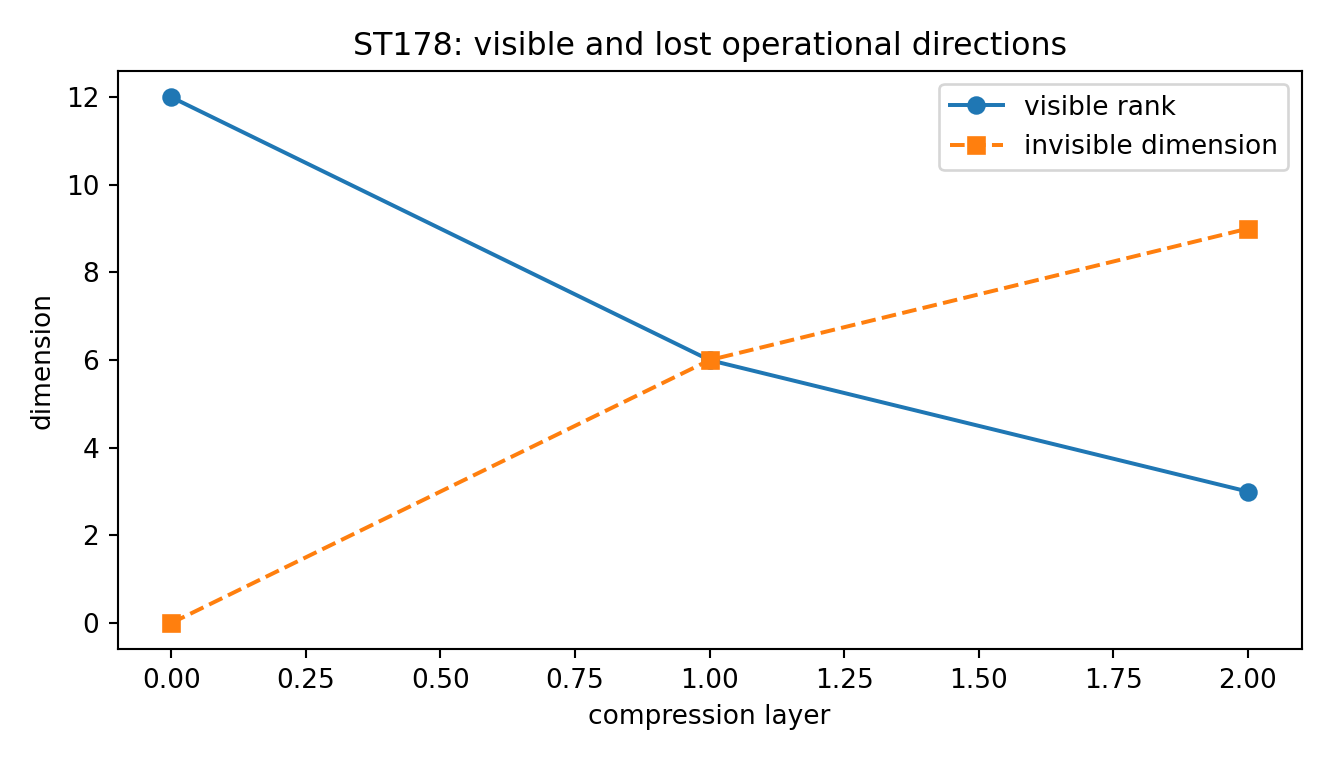
\includegraphics[width=.72\textwidth]{FIN_ST178_ST189_Figures/st178_irreversible_carriers.png}
\caption{ST178. Each hard coarse-graining decreases visible rank and enlarges the exact blindness subspace.}
\end{figure}

This is the correct irreversible generalization of ST166. Reversible carriers preserve a complete operational table; irreversible carriers preserve only a sufficient statistic determined by the quotient map.

\section{ST179: a state-dependent interaction outside strict functional calculus}

Define
\[
L_\rho=\operatorname{diag}\!\bigl(\operatorname{diag}(A\rho A)\bigr).
\]
This map is nonlinear in the pair $(A,\rho)$ as an interaction-selection rule and is generally not a spectral function $f(A)$. For every cyclic shift $R$,
\[
L_{R\rho R^*}=R L_\rho R^*.
\]

\begin{theorem}[Conditional state-to-pointer compiler]
For $\rho=I/12$, $L_\rho$ is scalar and its commutant has dimension $144$. A localized vertex state leaves seven distance values and a $22$-dimensional commutant. The supplied generic asymmetric full-support state gives twelve distinct values and therefore a $12$-dimensional diagonal pointer commutant.
\end{theorem}

\begin{figure}[H]\centering
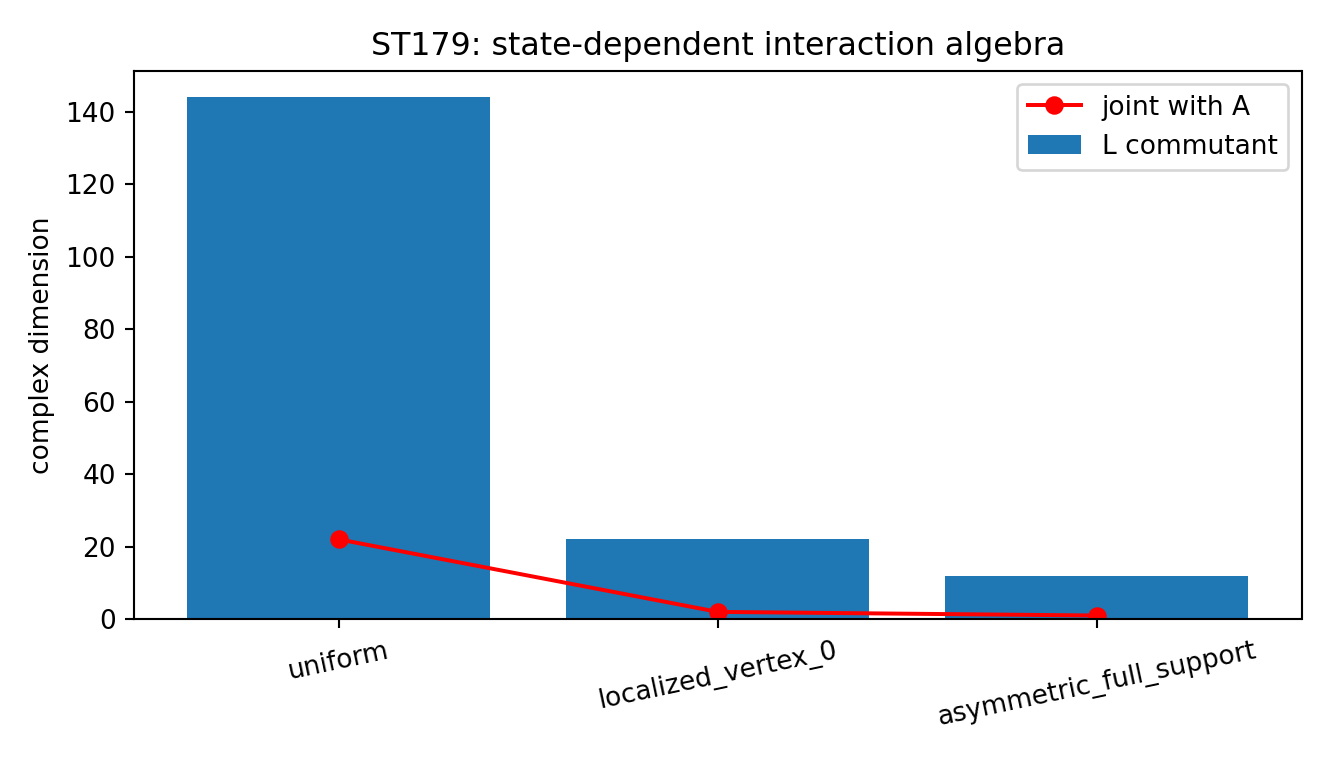
\includegraphics[width=.73\textwidth]{FIN_ST178_ST189_Figures/st179_state_interaction.png}
\caption{ST179. The state-dependent interaction translates increasing state asymmetry into a finer pointer algebra. Joint inclusion of $A$ leaves a smaller fixed algebra.}
\end{figure}

The result escapes the ST167 class but not the selector obstruction. The uniform state does nothing. The asymmetric state already carries the missing choice. Moreover, the displayed joint commutant of $A$ and generic $L_\rho$ is scalar, so simultaneous coherent strict evolution and exact pointer preservation require an additional dynamical design.

\section{ST180: sixty interval-certified departures from uniform folds}

ST168 proved 30 uniform reflection-even fold null lines: five stationary real amplitudes times six positive Fourier classes. For each fold $(q_0,\kappa_0,v)$, ST180 imposes the signed slice
\[
\langle v,q-q_0\rangle=\epsilon,
\qquad \epsilon=\pm10^{-3},
\]
and solves the seven stationary equations together with this slice constraint.

\begin{theorem}[Validated signed continuation]
All $30\times2=60$ square systems possess exactly one root in their accepted Krawczyk boxes. Every root is nonuniform. The smallest strict inclusion margin is
\[
9.966522740434414\times10^{-8}>0.
\]
The proof is uniform over the outward transcendental enclosure of the strict operator.
\end{theorem}

\begin{figure}[H]\centering
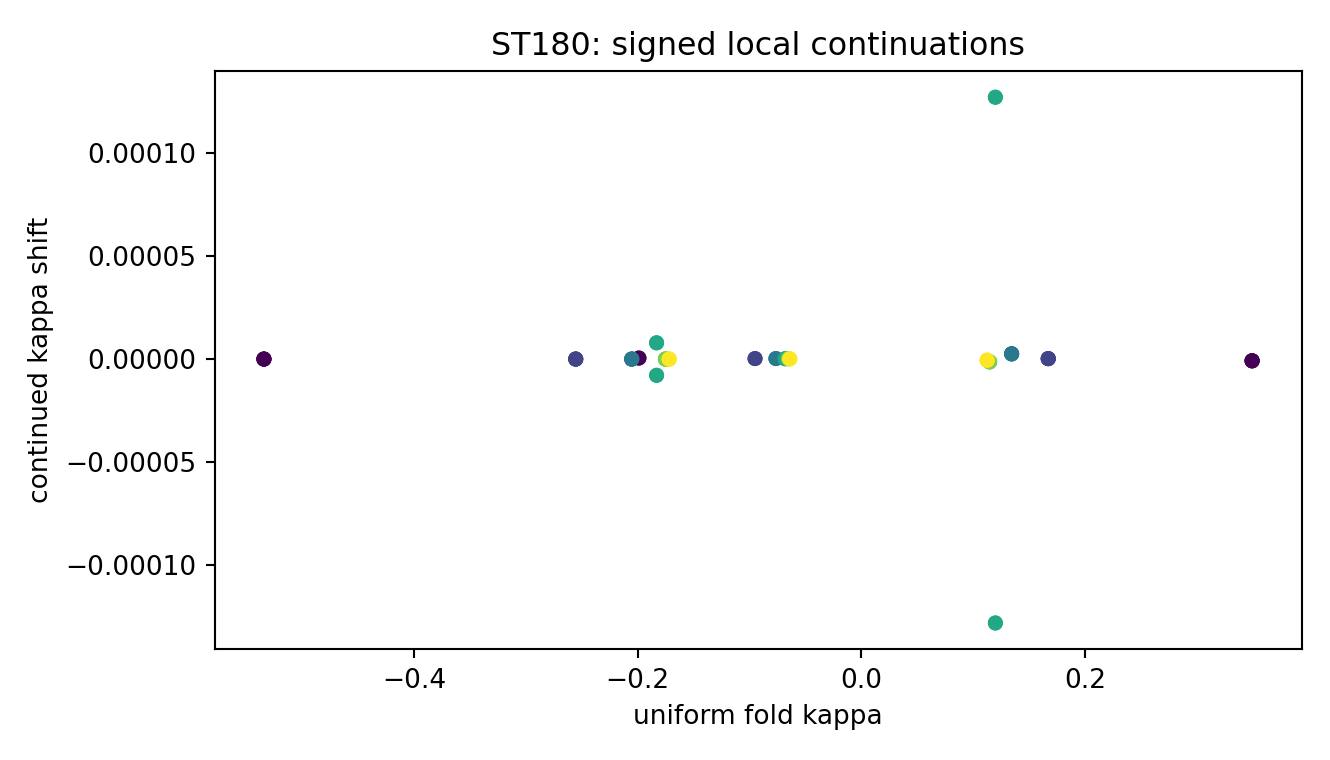
\includegraphics[width=.74\textwidth]{FIN_ST178_ST189_Figures/st180_fold_continuation.png}
\caption{ST180. Parameter displacement of the two signed local stationary states adjacent to every exact uniform fold.}
\end{figure}

This is a genuine advance from isolated uniform folds to rigorously existing nonuniform stationary states. It remains local: the slice, reflection sector, and distance are fixed, and no global branch connectivity, collision, orbital stability, or physical phase transition is asserted.

\section{ST181: three nonorthogonal commuting phase errors}

In syndrome branch $y$, let the three subnormalized phase-error weights be $w_{a|y}$ with phases $\theta_a$. Define
\[
W_y=\sum_aw_{a|y},\qquad c_y=\sum_aw_{a|y}e^{i\theta_a}.
\]

\begin{theorem}[Finite commuting phase recovery]
For any finite family of commuting qubit $Z$-phase errors,
\[
F_{e,y}^{*}=\frac{W_y+|c_y|}{2},\qquad
F_e^*=\sum_yF_{e,y}^{*}.
\]
The primal phase correction aligns $c_y$. The conic dual certificate is
\[
|c_y|=\min\left\{t:\begin{pmatrix}t&c_y\\c_y^*&t\end{pmatrix}\succeq0\right\},
\]
whose optimal slack eigenvalues are $0$ and $2|c_y|$.
\end{theorem}

The normalized three-error noisy-readout example gives
\[
F_e^*=0.947717686823979.
\]

\begin{figure}[H]\centering
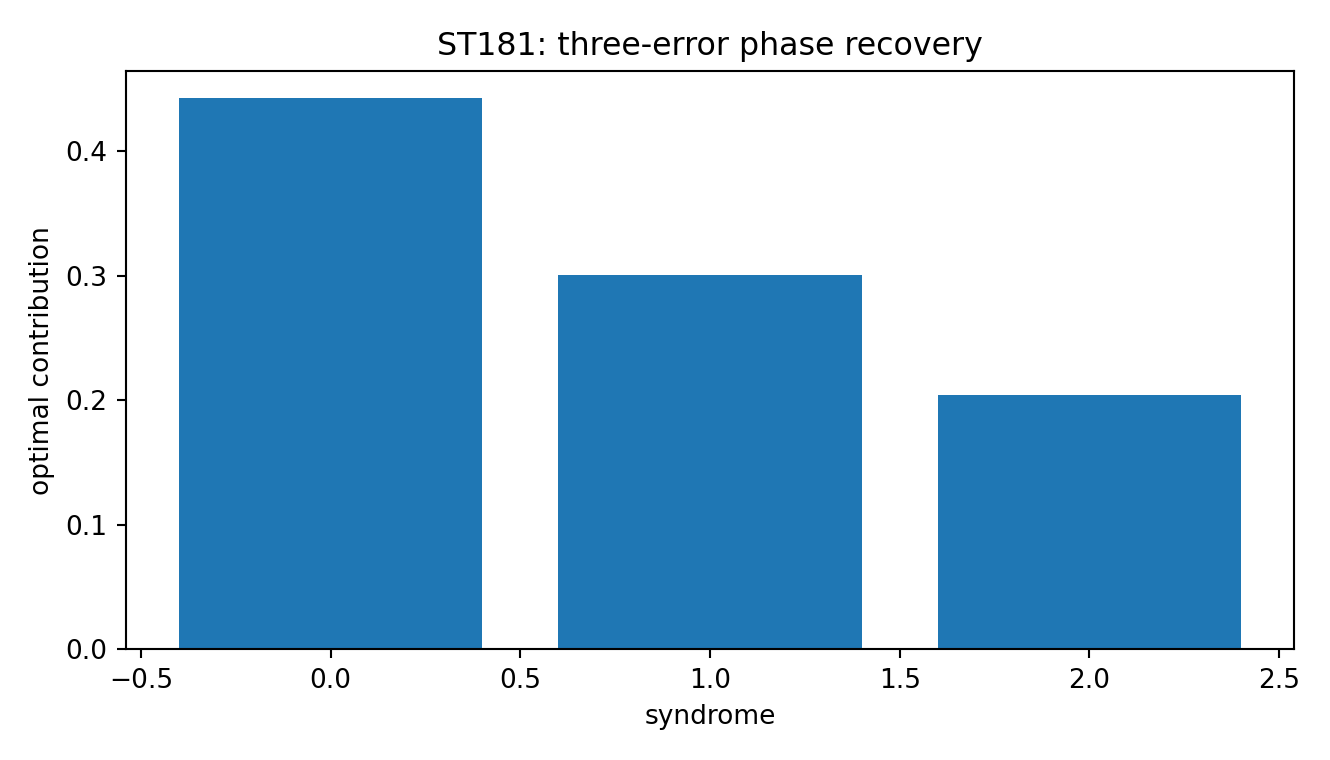
\includegraphics[width=.69\textwidth]{FIN_ST178_ST189_Figures/st181_three_error_recovery.png}
\caption{ST181. Certified optimal contribution of each noisy syndrome.}
\end{figure}

The theorem extends beyond three errors but requires a common qubit phase axis. Generic noncommuting errors retain a genuine semidefinite recovery problem.

\section{ST182 and ST183: controlled selection and a measurable nonlinear coefficient}

\subsection{A detailed-balance selector model}

Supply one preferred vertex with energies $E_0=-h$, $E_j=0$ and rates
\[
q_{i\to j}=\gamma\exp\!\left[-\frac\beta2(E_j-E_i)\right].
\]
These rates satisfy detailed balance. Starting from uniform, permutation symmetry among the eleven nonpreferred vertices closes the dynamics.

\begin{theorem}[Exact controlled selector trajectory]
The probability gap between the preferred vertex and every other vertex is
\[
g(t)=g_\infty(1-e^{-rt}),
\]
where
\[
g_\infty=\frac{e^{\beta h}-1}{e^{\beta h}+11},\qquad
r=\gamma\left(e^{\beta h/2}+11e^{-\beta h/2}\right).
\]
Conversely,
\[
\beta h=\log\frac{1+11g_\infty}{1-g_\infty}.
\]
\end{theorem}

\begin{figure}[H]\centering
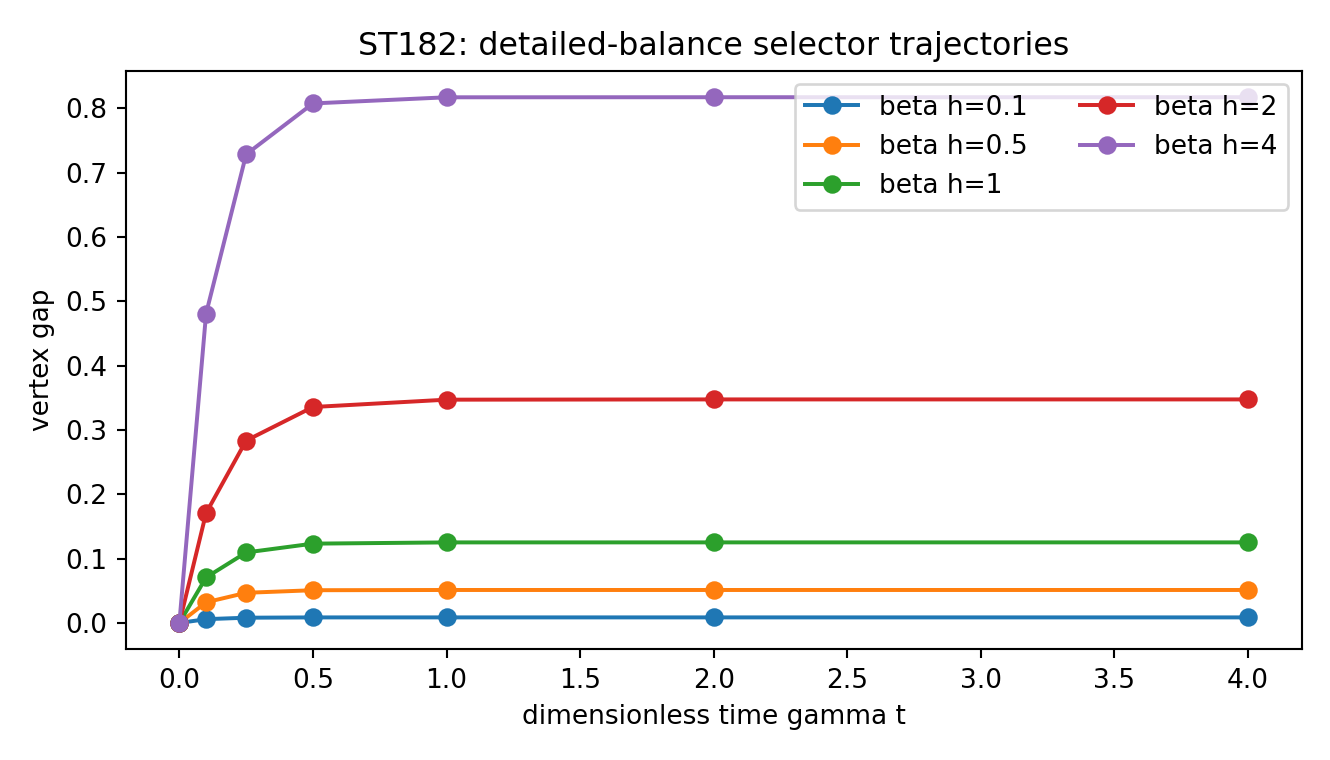
\includegraphics[width=.73\textwidth]{FIN_ST178_ST189_Figures/st182_selector_trajectories.png}
\caption{ST182. Exact dimensionless selector trajectories for five supplied fields.}
\end{figure}

\conditional{} This is not spontaneous symmetry breaking. The preferred vertex, energy field, bath temperature, rate scale, and clock are inputs.

\subsection{Two exact estimators of the missing degree-twelve coupling}

For
\[
V_g=V_0+\frac g{12}\sum_j\psi_j^{12},
\]
assuming $V_0$ has no local degree-twelve contribution,
\[
g=\frac1{11!}\frac{\partial^{12}V_g}{\partial\psi_j^{12}}(0).
\]
On the normalized first Fourier mode, if $[r^{12}\cos(12\theta)]V_g$ denotes the corresponding coefficient,
\[
g=2048\,6^6\,[r^{12}\cos(12\theta)]V_g.
\]

\begin{theorem}[Equivalent response identification]
The vertex twelfth derivative and first-mode angular response recover the same dimensionless $g$ exactly.
\end{theorem}

This closes identifiability once a nonlinear response is accessible. It does not source $g$ from the strict quadratic operator, assign physical units, or specify an experiment.

\section{ST184: the nuisance cube reaches halfwidth \texorpdfstring{$10^{-4}$}{1e-4}}

The complete cube
\[
|q_0-0.2|,\ |q_1-0.7|,\ |\delta-0.05|\le10^{-4}
\]
was partitioned into $7^3=343$ cells of halfwidth $10^{-4}/7$. Every cell passes interval Krawczyk inclusion. The smallest margin is
\[
9.526523284221211\times10^{-4}.
\]

\begin{theorem}[Third-generation uniform continuation]
The declared stationary branch exists uniquely throughout every cell of the complete 343-cell cover.
\end{theorem}

\begin{figure}[H]\centering
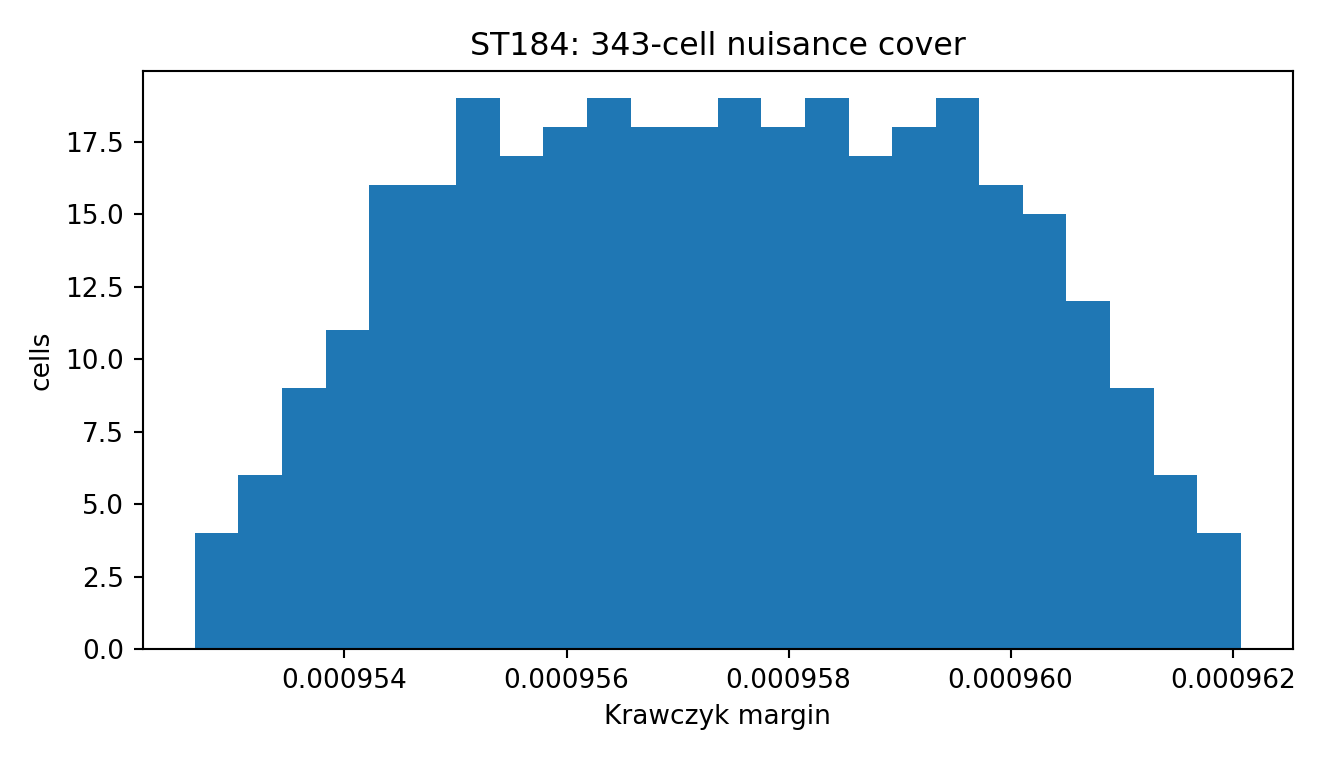
\includegraphics[width=.71\textwidth]{FIN_ST178_ST189_Figures/st184_cover.png}
\caption{ST184. Positive inclusion margins across the enlarged 343-cell cover.}
\end{figure}

This doubles the ST159 halfwidth and increases the ST172 halfwidth by one third. It does not locate the maximal continuation boundary or calibrate any physical tolerance.

\section{ST185: the Layer Visibility Spectrum}

This program directly tests the proposed intuition. Let
\[
C^{(n)}=C_nC_{n-1}\cdots C_1
\]
map a deep informational state to the observer's developed layer. Define the \emph{Layer Visibility Spectrum} (LVS) as the singular spectrum
\[
\operatorname{LVS}_n=\{\sigma_k(C^{(n)})\}_k.
\]

\begin{theorem}[Layered observation]
For each singular mode:
\begin{enumerate}
\item $\sigma_k=0$ means exact operational invisibility at the observing layer;
\item $\sigma_k>0$ permits noiseless algebraic recovery, but any inverse amplifies observation error by at least $1/\sigma_k$ in that mode;
\item total variation and relative entropy between any two states cannot increase under another stochastic layer.
\end{enumerate}
\end{theorem}

For a repeated translation-invariant soft layer
\[
B=(1-\epsilon)I+\frac\epsilon2(S+S^{-1}),qquad \epsilon=\frac14,
\]
the Fourier eigenvalues are
\[
\mu_k=1-\epsilon+\epsilon\cos(2\pi k/12),
\]
so after $n$ self-similar layers the visibility is exactly $|\mu_k|^n$.

\begin{figure}[H]\centering
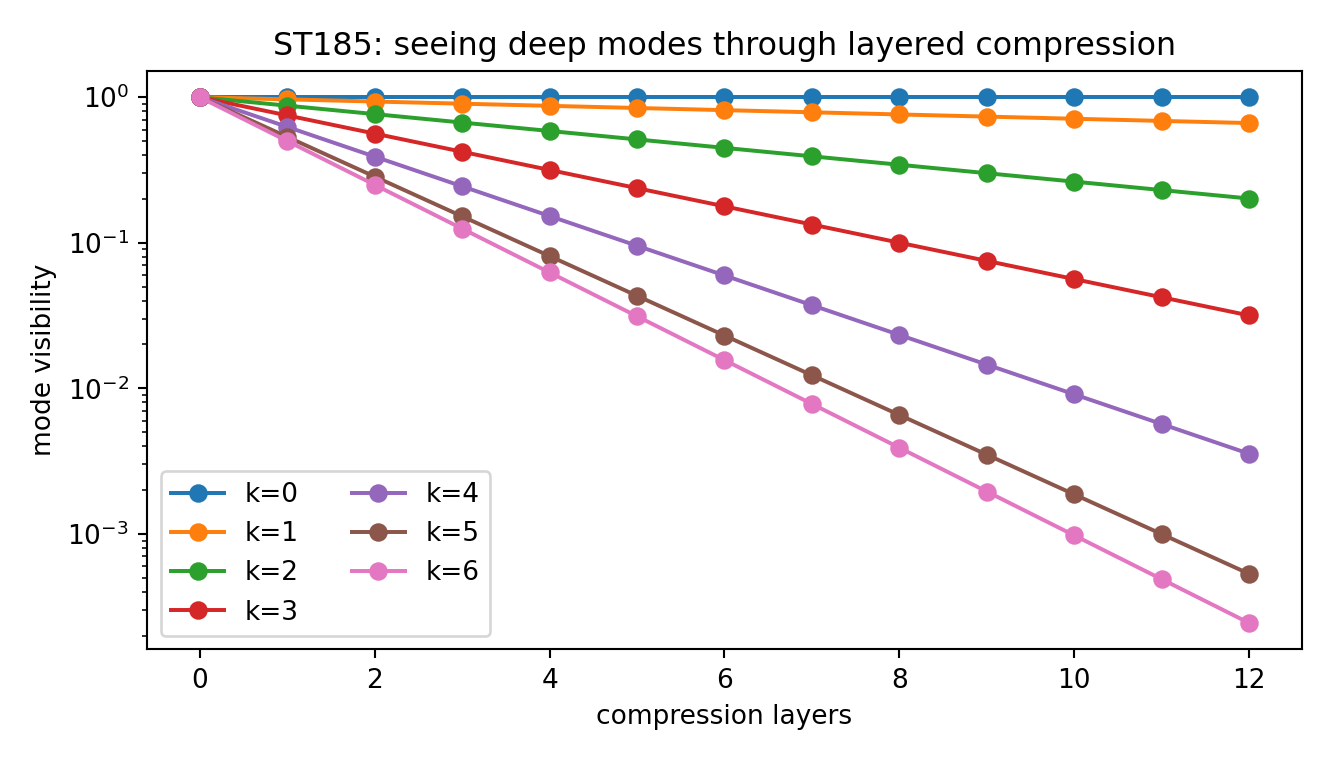
\includegraphics[width=.76\textwidth]{FIN_ST178_ST189_Figures/st185_layer_visibility.png}
\caption{ST185. Different deep Fourier modes survive repeated soft compression at exponentially different rates. The constant mode is preserved; the highest mode is suppressed fastest.}
\end{figure}

For $k=6$, $\mu_6=1/2$. At twelve layers,
\[
\sigma_6=2^{-12}=0.000244140625,
\qquad \sigma_6^{-1}=4096.
\]
Thus the mode still exists mathematically in a noiseless observation, yet modest layer noise makes its reconstruction statistically prohibitive. Hard block compression instead sets nine directions exactly to zero.

\subsection{Interpretation of the intuition}

The hypothesis now separates into three distinct cases:

\begin{enumerate}
\item \textbf{Transparent deep scale:} the relevant singular value is near one, so the developed layer sees it almost directly.
\item \textbf{Shadow of a deep scale:} the singular value is nonzero but small; the observer sees an attenuated image requiring rapidly growing samples to reconstruct.
\item \textbf{Quotiented deep scale:} the singular value is zero; no measurement confined to the developed layer can distinguish changes along that mode.
\end{enumerate}

This gives a rigorous meaning to ``seeing lower scales through fractal layers.'' However, the adjective \emph{fractal} is justified here only by repeated/self-similar composition. A geometric fractal dimension, physical length ratio, Planck cell, renormalization fixed point, and map from layer number to experimentally measured scale remain absent.

\section{ST186: exact factors, noisy subspaces, and gauge ambiguity}

For two complete commuting $M_2$ factors generating $M_4$, finite-dimensional algebra theory gives a unitary $U$ carrying them to
\[
M_2\otimes I,qquad I\otimes M_2.
\]

\begin{theorem}[Factor classification]
Labeled commuting $M_2$ factors generating $M_4$ determine the tensor-factor pair up to a global conjugation whose residual freedom is local $U(2)\times U(2)$. If labels are removed, factor swap is an additional ambiguity.
\end{theorem}

The commutator Laplacian of complete noiseless generators has a four-dimensional zero eigenspace and gap four. With generic noise, the four-dimensional low subspace remains close but ceases to be exactly closed under multiplication.

\begin{figure}[H]\centering
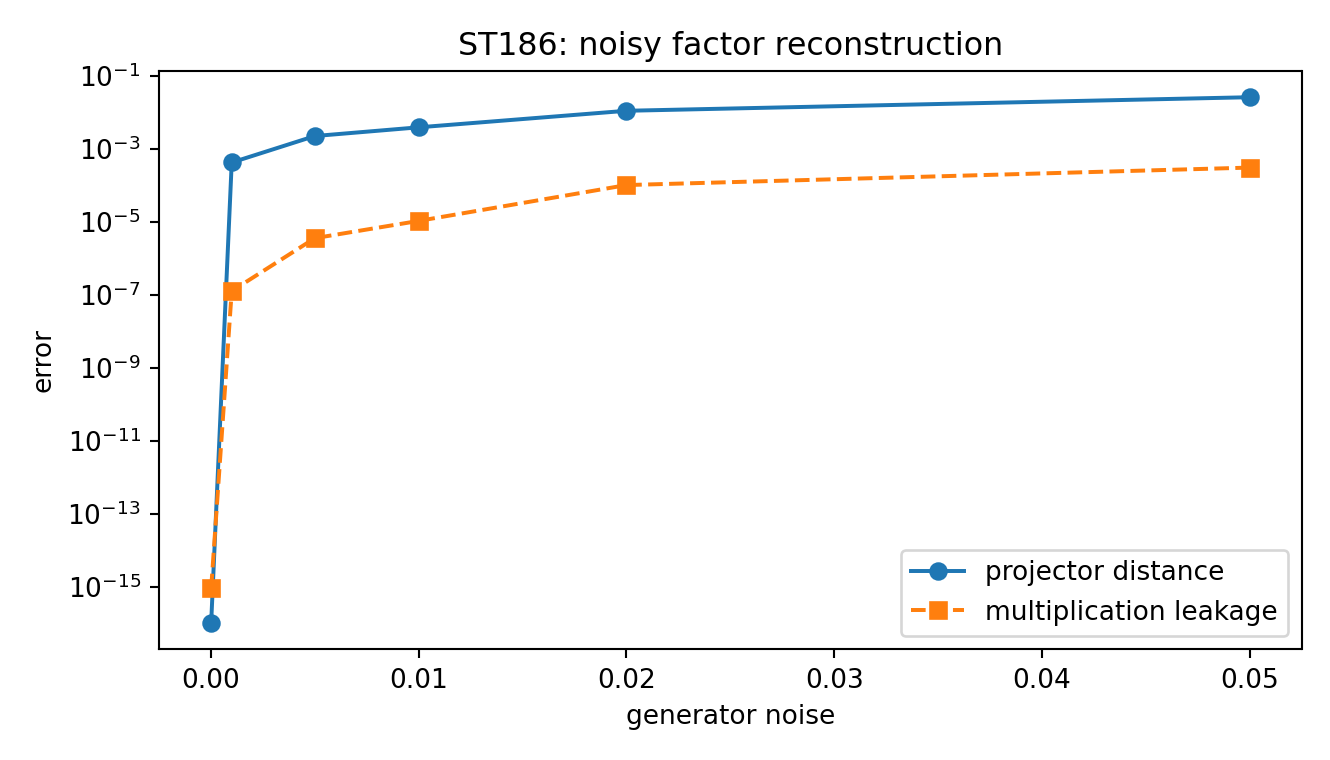
\includegraphics[width=.72\textwidth]{FIN_ST178_ST189_Figures/st186_factor_recovery.png}
\caption{ST186. Noisy low-subspace displacement and multiplication leakage. The curve is a seeded numerical audit; the noiseless classification is exact.}
\end{figure}

Therefore noisy spectral recovery alone does not produce an exact algebra. Projection onto the matrix-factor variety, label recovery, and physical subsystem interpretation are separate estimation problems.

\section{ST187: how loose is the pair-path hidden-HMM bound?}

Let $Z_n$ be the observed Hellinger coefficient obtained by summing over all $2^n$ binary records. Let $B_n$ be the pair-hidden-path coefficient used by ST162/ST175.

\begin{theorem}[Finite observed/pair inequality]
For every finite $n$,
\[
Z_n\le B_n.
\]
This follows from the same concavity/subadditivity expansion that produces the pair-path transfer matrix.
\end{theorem}

Complete deterministic forward enumeration gives, at $n=20$,
\[
Z_{20}=3.616302630613104\times10^{-7},\qquad
B_{20}=0.0015695570497458744,
\]
and hence
\[
\frac{B_{20}}{Z_{20}}=4340.225943645024.
\]
The corresponding finite rates are $0.7416321759918023$ and $0.3228480916674504$.

\begin{figure}[H]\centering
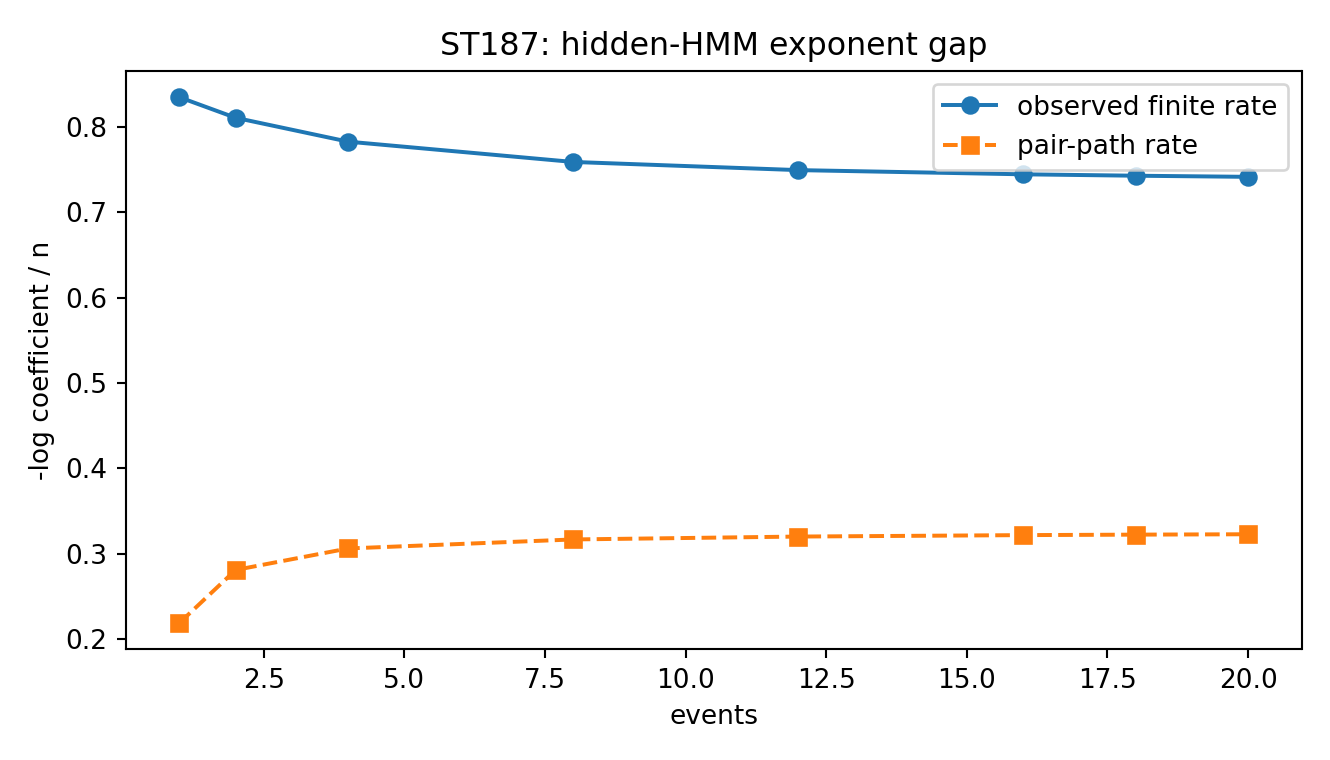
\includegraphics[width=.72\textwidth]{FIN_ST178_ST189_Figures/st187_hmm_gap.png}
\caption{ST187. The rigorous pair-path exponent remains positive but is quantitatively conservative.}
\end{figure}

\strong{} The trend strongly suggests a nonzero asymptotic gap. The enumerated values are floating finite-$n$ audits, not an interval transfer-operator proof of the exact observed asymptotic Chernoff rate.

\section{ST188: local circuits versus energy-conserving generators}

Embed the strict $12\times12$ operator in the leading block of a four-qubit register, with four zero padding states. For identical system and bath registers, the global register SWAP $S_{\rm reg}$ obeys exactly
\[
[S_{\rm reg},H\otimes I+I\otimes H]=0.
\]
It is also the product of four disjoint pairwise qubit SWAPs.

The four individual two-qubit SWAP generators do not separately conserve the encoded energy. Their commutator Gram matrix has numerical eigenvalues
\[
212.00756,\quad225.78523,\quad329.49044,\quad329.49044.
\]

\begin{figure}[H]\centering
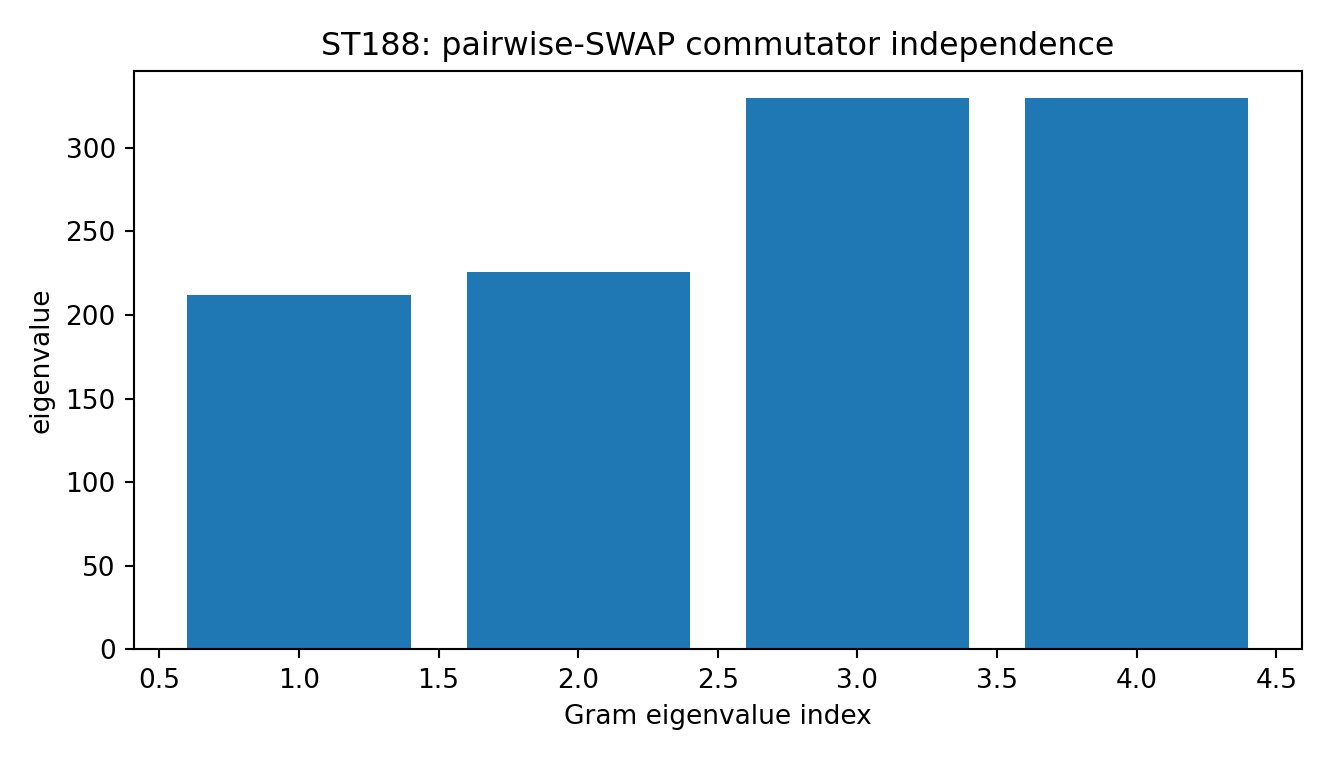
\includegraphics[width=.68\textwidth]{FIN_ST178_ST189_Figures/st188_swap_gram.png}
\caption{ST188. Positive numerical Gram spectrum for the four static pairwise-SWAP commutators.}
\end{figure}

\strong{} Within this padded encoding and four-dimensional static generator span, no nonzero linear combination commutes with total energy. This is not a universal no-go: time-dependent controls, ancillary systems, other two-local interactions, different encodings, and an interval rank certificate remain open.

\section{ST189: a validator that cannot manufacture external evidence}

The external interface accepts a JSONL event file and prior registration. Required event fields are
\[
\{\texttt{timestamp,outcome,config,run\_id}\}.
\]
It checks the exact file hash, holdout hash, a frozen-before-unblinding flag, and distinct provider/registrar/analyst labels. Physical validity additionally requires an external path, calibration hash, independent-custody attestation, and laboratory-execution attestation.

The synthetic clean packet returns
\[
\boxed{\texttt{EXTERNAL\_RECORD\_STRUCTURALLY\_VALID\_PHYSICAL\_ATTESTATION\_BLOCKED}}.
\]
Appending one byte invalidates the file hash and the structural packet.

\begin{theorem}[Executable evidence boundary]
The interface detects the declared tampering and refuses physical promotion when external attestations are absent. It cannot verify human identity, create custody, certify calibration, or prove that laboratory events occurred.
\end{theorem}

No external event record was supplied or analyzed in this release.

\section{Combined interpretation and falsification}

The new layer theorem supports a constrained version of the proposed picture:
\[
\text{deep nadsoliton information}
\xrightarrow{C_1}\text{layer 1}
\xrightarrow{C_2}\cdots
\xrightarrow{C_n}\text{observer statistics}.
\]
It explains mathematically how many different deep configurations can cast the same observational shadow, why some high-frequency structure is exponentially difficult to recover, and why coarse-level entropy or spectra cannot reconstruct all fine geometry.

It does \emph{not} establish the following stronger chain:
\[
\text{strict FIN kernel}\Longrightarrow
\text{unique fractal hierarchy}\Longrightarrow
\text{spacetime/matter}\Longrightarrow
\text{our measurements}.
\]
The first implication lacks a sourced hierarchy map. The second lacks a dimensional and physical bridge. The third lacks preparations, instruments, environment, apparatus, and independently registered data.

\subsection{What the results falsify}

\begin{itemize}
\item A developed layer cannot recover directions in the exact kernel of its composite observation map.
\item Nonzero deep modes are not automatically observable in practice: inverse noise amplification may grow exponentially with layer count.
\item The ST179 nonlinear interaction does not spontaneously select from the uniform state.
\item The ST175 pair-path exponent is not quantitatively close to the enumerated observed finite rate in the supplied HMM.
\item A depth-one product of local SWAP gates does not imply that its static two-local generator conserves an interacting encoded energy throughout the path.
\end{itemize}

\subsection{What remains open}

The highest-value missing theorem is now:
\begin{quote}
derive a nontrivial hierarchy $C_1,C_2,\ldots$ from the informational nadsoliton itself, prove an appropriate self-similarity/refinement law, and identify operational observables that survive to a calibrated physical layer.
\end{quote}
Such a theorem must not silently import the legacy Planck hierarchy, a selector, or physical units.

\section{Recommended next programs ST190--ST202}

\begin{longtable}{@{}p{0.08\textwidth}p{0.12\textwidth}p{0.72\textwidth}@{}}
\toprule Program & Priority & Executable target\\\midrule\endfirsthead
\toprule Program & Priority & Executable target\\\midrule\endhead
ST190 & 1 & Derive one repository-sourced hierarchy-map candidate and test its Layer Visibility Spectrum without importing a Planck scale.\\
ST191 & 2 & Classify irreversible carrier equivalence by Blackwell sufficiency and minimal sufficient operational quotients.\\
ST192 & 3 & Supply a dynamics for the ST179 interaction and prove or refute spontaneous pointer selection from symmetric noise.\\
ST193 & 4 & Perform validated arclength continuation and branch-collision search beyond the fixed ST180 slices.\\
ST194 & 5 & Solve three generic noncommuting qubit errors with rational primal--dual SDP certificates.\\
ST195 & 6 & Optimize time-dependent detailed-balance selector controls under a frozen entropy-production budget.\\
ST196 & 7 & Search internal dimensionless laws relating ST183 response estimators to a strict nonlinear source.\\
ST197 & 8 & Locate the maximal nuisance continuation boundary by adaptive interval branch-and-bound.\\
ST198 & 9 & Derive sample-complexity lower bounds for attenuated deep modes under Poisson and multinomial noise.\\
ST199 & 10 & Project noisy commutant subspaces onto the nearest exact matrix-factor variety with uniqueness certificates.\\
ST200 & 11 & Certify the exact observed hidden-HMM Hellinger rate using an interval transfer operator on belief space.\\
ST201 & 12 & Interval-certify or falsify the ST188 restricted ansatz rank and enlarge the local generator class.\\
ST202 & 13 & Execute ST189 only on a genuinely external immutable record with independently supplied custody attestations.\\
\bottomrule
\end{longtable}

ST190 has the greatest conceptual leverage because it tests whether the new visibility architecture belongs to FIN rather than merely being compatible with it. ST191 and ST198 then determine what information and sample resources an observer at a coarse layer can recover. ST192 remains the sharpest selector test.

\section{Reproducibility}

The release package contains:
\begin{itemize}
\item \texttt{fin\_st178\_st189\_research.py}: all twelve studies and ten figures;
\item \texttt{fin\_st189\_external\_record\_validator.py}: external-record interface and synthetic tamper test;
\item \texttt{test\_fin\_st178\_st189.py}: 29 live and serialized tests;
\item \texttt{FIN\_ST178\_ST189\_Results.json}, summary CSV, and twelve specialized JSON packets;
\item \texttt{FIN\_ST178\_ST189\_SHA256SUMS.txt}: release manifest.
\end{itemize}

Seed \texttt{20260826} controls the ST185 data-processing example and ST186 noisy subspace audit. The core range/kernel theorem, Fourier visibility formula, interval fold and nuisance certificates, response identities, and global-SWAP commutation do not depend on that seed. ST187 uses complete binary-record enumeration through $n=20$ but floating arithmetic; its exact asymptotic rate remains open.

\section{Final conclusion}

The intuition motivating this release survives a serious mathematical test in a restricted form. If physical observation is mediated by a sequence of compression maps, then an observer on a developed layer necessarily sees only a quotient of the deeper information. Some deep modes survive as stable observables, some appear only as exponentially attenuated shadows, and some are exactly erased. This is not metaphor: it follows from the range, kernel, and singular spectrum of the composite observation map.

The same analysis also identifies the obstruction. Neither the strict operator nor the current legacy-to-strict bridge exports the hierarchy maps. Self-similar repetition can be constructed, but its layer count has no derived conversion to length, energy, or time. Consequently the theory cannot yet say which layer corresponds to our physics, whether lower scales are spatial or merely informational, or whether the hierarchy generates matter and geometry.

\resultbox{\textbf{Deepest surviving interpretation after ST178--ST189.} FIN can consistently be extended to a multiscale operational architecture in which observed physics is a compressed shadow of deeper nadsoliton information. The invariant mathematical object is the hierarchy of statistical maps together with its Layer Visibility Spectrum. This architecture rigorously explains visibility, attenuation, exact blindness, and reconstruction cost. Its application to our universe remains conditional until FIN derives the hierarchy, a selector, dimensions, and a realized operational bridge.}

\vfill
\hrule
\smallskip
\textbf{Author metadata:} Krzysztof \.{Z}uchowski; Independent Researcher --- Fractal Information Theory Project; ORCID 0009-0002-0909-3613. Release 10.69, version 1.0.0, August 11, 2026. CC BY 4.0.

\end{document}
